\clearpage
\chapter{Vorgehensweise}
\section{Task-Technology-Fit Theory}

Das Ziel dieser Projektarbeit ist es, die Eignung der SAP BTP als digitale Plattform für Kfz-Versicherer zu untersuchen. Hierfür sollen zunächst die Anforderungen der Kfz-Versicherer an technische Plattformen identifiziert und anschließend mit den Funktionen und Services der SAP Business Technology Platform verglichen werden.

Zur Unterstützung dieser Analyse wird das in Abbildung …  dargestellte Task-Technology-Fit (TTF) Modell (TTF) von Goodhue und Thompson verwendet. Es vergleicht die Charakteristiken einer bestimmten Aufgabe mit den Charakteristiken einer bestimmten Technologie, die zur Erfüllung der Aufgabe verwendet werden soll. Gemäß Goodhue et. al (1995) kann eine Technologie nur dann eine positive Auswirkung auf die Leistung von Einzelpersonen oder Organisationen haben, wenn eine Übereinstimmung zwischen den Funktionalitäten der Technologie und den Anforderungen der Nutzer besteht. Die Leistungen werden umso positiver beeinflusst, je besser die Technologie mit der zu unterstützenden Aufgabe übereinstimmt. \autocite[Vgl.][S. 214-216]{GOODHUE1995} Hierbei kann die TTF-Analyse auf verschiedenen Abstraktionsebenen durchgeführt werden, da die Vorteile der Verbesserung der Produktivität nicht nur auf Einzelpersonen, sondern auch auf ganze Organisationen übertragen werden können.\autocite[Vgl.][S. 1827f]{GOODHUE1995b} Eine verbesserte Leistung kann gemäß TTF auf die reibungslose Ausführung der Aufgabe, die Verringerung der Kosten für die Ausführung der Aufgabe oder die Erleichterung der Aufgabe zurückzuführen. \autocite[Vgl.][S. 96]{LEE2007}

\autocite[Vgl.][S. 215]{GOODHUE1995}
\autocite[Vgl.][S. 399]{SPIES2020}

\begin{figure}[h]
    \centering
    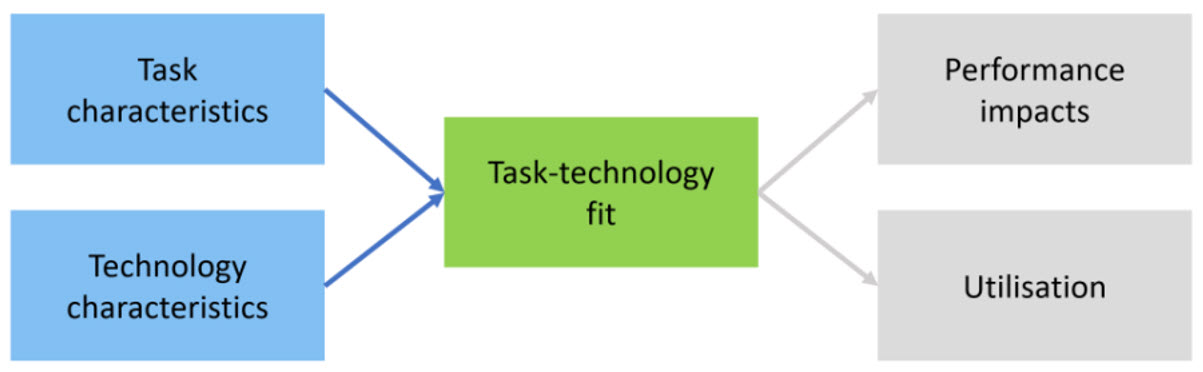
\includegraphics[width=1\textwidth]{img/TTF_Nadine.jpg}
    \caption[Modell der Task-Technology-Fit Theorie]{Modell der Task-Technology-Fit Theorie\autocite{TTF}}
    \label{fig:TTF}
\end{figure}
\footnotetext{Vgl. eigene Darstellung angelehnt an: Hahn, 2016, S. 599 und Beimborn et al., 2011, S. 372.}

\improvement{Frage ob man hier die Grafik mit Utilization nimmt und später ausgrenzt oder direkt eine andere Grafik nimmt}

Die Task Charakteristiken beziehen sich auf die Gesamtheit der physischen und kognitiven Handlungen und Prozesse, die von einer Organisation oder einer Einzelperson in einer bestimmten Umgebung ausgeführt werden. Sie werden speziell in Bezug zur Technologie, welche sie bei der Ausführung unterstützen soll, betrachtet und je nach Komplexität auf unterschiedliche Detailebenen heruntergebrochen. \autocite[Vgl.][S. 398]{SPIES2020} Die zur Evaluation der Technologie notwendigen Anforderungen können nach Goodhue 1998 durch ein Task-Model, Literaturrecherche oder mittels Interviews erhoben werden. \autocite[Vgl.][S. 126]{GOODHUE1998} In dieser Kontext wird eine Anforderung definiert als eine Aussage, „die einen Bedarf und die damit verbundenen Einschränkungen und Bedingungen umsetzt oder ausdrückt“. \autocite[Vgl.][]{ISO2017}

Als Technologie Charakteristiken werden im Rahmen des TTF Models die Werkzeuge bezeichnet, welche von Einzelpersonen zur Ausführung ihrer Aufgaben oder zur Unterstützung bei der Ausführung ihrer Aufgaben verwendet werden sollen.\autocite[Vgl.][S. 216]{GOODHUE1995}. Dabei ist das Modell so allgemein gehalten, dass es entweder auf die Auswirkungen eines bestimmten Systems oder auf die allgemeineren Auswirkungen der Gesamtheit der bereitgestellten Systeme, Strategien und Dienste ausgerichtet sein kann. \autocite[Vgl.][S. 399]{SPIES2020}




\newpage
\section{Systematische Literaturanalyse}
\newpage
\section{Semistrukturierte Leitfadeninterview}
\newpage